\documentclass[11pt]{article}
\usepackage[utf8]{inputenc}
\usepackage{HBSuerDemir}
\usepackage{caption}
\usepackage{wrapfig}

\title{b2p1-204}
\author{hkubraeryilmaz }
\date{November 2016}

\begin{document}
\hPage{b2p1/204}

b) Having \(Q\bigg(\dfrac{x+0}{1+t}\ , \ \dfrac{y+0}{1+t} \ , \ \dfrac{z+t}{1+t}\bigg) \) on the generatrix, and setting its coordinates on $F=0, \ G=0$ :
\[
    \bigg(\dfrac{x}{1+t}\bigg)^2 \ = \ 2 \ \dfrac{z+t}{1+t} \ , \qquad \frac{y}{1+t} \ - \ \frac{z+t}{1+t} \ = \ 1 
\]

\begin{align*}
    \Rightarrow &x^2 \quad = \ 2(1+t)(z+t), \qquad y-(z+t) \ = \ 1+t \\
    \Rightarrow &x^2 \quad = \ 2(1+t)(z+t), \qquad 2t=y-z-1 \\
    \Rightarrow &x^2 \quad = \ (2+y-z-1)\bigg(z+ \dfrac{y-z-1}{2} \bigg) \\
    \Rightarrow &2x^2 \; = \ (y-z+1)(y+z-1) \\
    \Rightarrow &2x^2 \; = \ y^2 - (z-1)^2 \\
    \Rightarrow &2x^2-y^2+z^2-2z+1 \ = \ 0 
\end{align*}

\underline{3. Surfaces of revolution}: 

A surface S generated when a curve $\Gamma$ is revolved about a line $\Delta$ is called a \underline{surface of revolution}. 

\begin{wrapfigure}{r}{0.4\linewidth}
    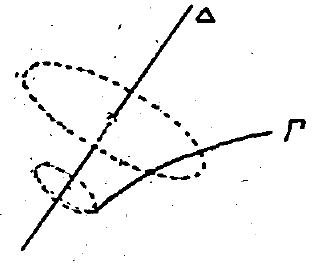
\includegraphics[width=\linewidth]{images/b2p1-204-fig01.png}
    \caption*{}
\end{wrapfigure}

$\Gamma$ is the \underline{generatrix} and $\Delta$ is the \underline{axis} of the surface, and we say that S is defined by $\Delta$ and  $\Gamma$.  

Spheres, right circular cylinders and cones are examples of surface of revolution.

Every point of $\Gamma$ describes a circle with the center on the axis $\Delta$ , called a \underline{"parallel"} , and any plane through $\Delta$ intersects the surface along a curve called a \underline{"meridian"} of S.

The meridians are congruent curves of S, and S may be generated by revolving any meridian about the axis $\Delta$ .

An equivalent definition of a surface of revolution is the following: A surface of revolution is the locus of a variable circle with given axis $\Delta$ and subject to another condition such as

\end{document}